\subsection{Verhalten}

Eine Änderung des Zustands eines Objektes, wie zum Beispiel der schon angesprochene Farbwechsel von Marvins Auto aus Abbildung~\ref{fig:Abb-3-8} von rot zu grün, wird durch die Ausführung von Operationen durchgeführt, die durch die entsprechende Klasse für ihre Instanzen definiert wurden. Operationen spezifizieren, welche Funktionalität ein Objekt (für andere Objekte des Systems) anbietet. Man verwendet in diesem Zusammenhang auch den Begriff Dienstleistung und beschreibt mit den Begriffen Dienstleister und Dienstnutzer, welche Rolle ein Objekt bei Ausführung einer bestimmten Operation einnimmt. Das Objekt, das eine Operation aufruft, ist der Dienstnutzer und das Objekt, dessen Operation aufgerufen wird, ist der Dienstleister. Die entsprechende Operation (bzw. die Funktionalität, die sie abbildet) ist dementsprechend der Dienst. Die reine objektorientierte Modellierung abstrahiert von dieser technischen Ebene der Operationsaufrufe und verwendet die Metapher des Nachrichtenversands bzw. des Austauschens von Botschaften zwischen Objekten: Ein Objekt sendet eine Nachricht an ein anderes Objekt. Das die Nachricht empfangende Objekt reagiert entweder entsprechend seiner definierten Verhaltensweisen oder reagiert nicht, wenn es für die Nachricht keine definierten Verhaltensweisen besitzt. Das Konzept des Nachrichtenaustausches zwischen Objekten orientiert sich an der Realwelt, in der Realwelt-Objekte verbal oder nonverbal Botschaften an andere Realwelt-Objekte übermitteln (z.B. die Aufforderung einer Mutter an ihr Kind das Zimmer aufzuräumen oder der fast-verhungernde Blick eines Hundes zu seinem Herrchen) und letztere auf bestimmte Art und Weise reagieren. Der Austausch von Nachrichten zwischen den Objekten in einem Softwaresystem bleibt in letzter Instanz aber doch eine Folge von Operationsaufrufen und Operationsausführungen.\footnote{@Cajus: Sätze schreiben: bei verteilten Systemen können es tatsächlich Nachrichten sein, Java und CORBA-Protokoll + @Maren: nachgucken, warum Smalltalk diese Nachrichten-Metapher gewählt hat und ob es bei Smalltalk etwas anderes ist als Operationsaufrufe} 
\begin{wrapfigure}{o}[70pt]{0.6\textwidth}
	%\vspace{-10pt}
	\centering 
	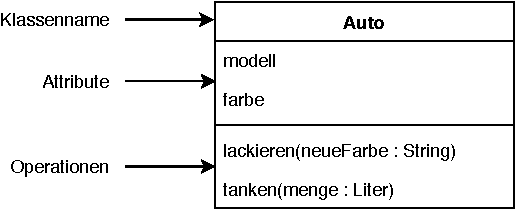
\includegraphics{../grafiken/Kapitel-3/Abb-3-11.pdf}
	\caption{Eine Klasse Auto mit Attributen und Operationen}
	\label{fig:Abb-3-11}
	\vspace{-6pt}
\end{wrapfigure}
Die Nachricht des Sender-Objektes besteht aus einem Operationsnamen und gegebenenfalls zusätzlichen Informationen in Form von Parametern. Das Empfänger-Objekt kann auf diese Nachricht genau dann reagieren, wenn eine entsprechende Operation definiert ist.\footnote{Objektorientierte Programmiersprachen verlangen in der Regel, dass nur Nachrichten gesendet werden, auf die ein Objekt auch reagieren kann. In compilierten Sprachen achtet darauf schon der Compiler. In Interpreter-Sprachen lösen solche Nachrichten Laufzeit-Fehler aus. Der Fall, dass ein Objekt eine Nachricht nicht verstehen kann, wird also im Gegensatz zur Realwelt nicht als gültige Möglichkeit angesehen.} Die Ausgestaltung der Operation bestimmt, was genau bei Eintreffen der Nachricht des Sender-Objektes passiert. Die Operationen, die das Verhalten der Objekte bestimmen, sind für alle Instanzen einer Klasse identisch. 
In der UML-Darstellung werden die Operationen dementsprechend auch in der Klasse notiert und nicht in den einzelnen Instanzen. Dafür wird das Rechteck der Klasse erneut horizontal unterteilt (Abb.~\ref{fig:Abb-3-11}).

Wie bei der Notation der Attribute kann die Angabe von Operationen in UML-Klassendiagrammen je nach Einsatzzweck des Modells mehr oder weniger detailliert sein. Ergänzend zu der minimalen Darstellung in Form des Operationsnamens können auch Eingangs- und/oder Rückgabeparameter oder auch zusätzliche textuelle Erläuterungen zu Implementierungserfordernissen mit angegeben werden. Für die Abbildung des Realwelt-Ausschnittes auf ein Domänenklassendiagramm genügen in der Regel die Operationsnamen.

Jede Instanz bietet genau die in ihrer Klasse definierten Operationen an. Die Reaktion auf einen entsprechenden Operationsaufruf kann aber (und wird meistens) abhängig vom Zustand der Instanz, auf der der Operationsaufruf durchgeführt wird sowie abhängig von den durch das aufrufende Objekt übergebenen Parametern unterschiedlich ausfallen. 
So ist es zum Beispiel sinnvoll, wenn eine Auto-Instanz, deren Tank leer ist, auf den Operationsaufruf tanken(30 Liter) anders reagiert als eine andere Auto-Instanz, deren Tank komplett gefüllt ist. Die Operationen, die ein Objekt anbietet, greifen daher in der Regel auf seine aktuellen Attributwerte zu. Man unterscheidet Operationen, die nur lesend auf Attribute zugreifen und deren Werte nicht verändern (Selektoren) und solche, die Attributwerte verändern, also (auch) schreibend auf Attribute zugreifen (Modifikatoren). Modifikatoren ändern also den Zustand eines Objektes, Selektoren tun dies nicht. Die Operation \texttt{lackieren(neueFarbe: String)} der Klasse \texttt{Auto} in Abbildung~\ref{fig:Abb-3-11} ist ein Beispiel für einen Modifikator, wenn wir sie so entwerfen, dass sie den Wert des Attributs \texttt{farbe} durch den Wert des übergebenen Parameters \texttt{neueFarbe} ersetzt. 
\begin{wrapfigure}{o}[70pt]{0.6\textwidth}
	%\vspace{-10pt}
	\centering 
	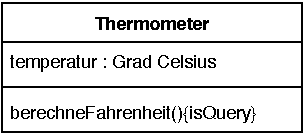
\includegraphics{../grafiken/Kapitel-3/Abb-3-12.pdf}
	\caption{Eine Klasse \texttt{Thermometer} mit Attribut und Selektor-Operation}
	\label{fig:Abb-3-12}
	\vspace{-6pt}
\end{wrapfigure}
Abbildung~\ref{fig:Abb-3-12} zeigt ein Beispiel für eine Selektor-Operation: Die Klasse \texttt{Thermometer} besitzt ein Attribut \texttt{temperatur}, das die Temperatur in der Einheit Grad Celsius enthält. Die Methode \texttt{berechneFahrenheit()} liest diesen Wert aus und errechnet daraus die Temperatur in der Einheit Grad Fahrenheit. In der UML können Selektor-Methoden über den Zusatz \{isQuery\} gekennzeichnet werden. Dieser Zusatz ist aber optional. Für viele Modellierungszwecke im Laufe der Softwareentwicklung ist es nicht relevant, ob eine bestimmte Operation in der späteren konkreten Implementierung ein Selektor oder ein Modifikator werden soll.

Die „einfachsten“ Selektor- und Modifikator-Operationen sind die (eingedeutscht so genannten) Getter und Setter. 
\begin{wrapfigure}{o}[70pt]{0.6\textwidth}
	%\vspace{-10pt}
	\centering 
	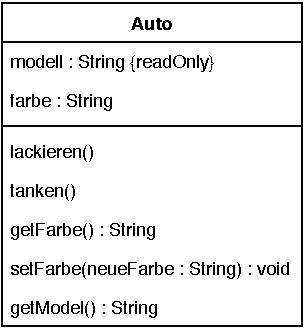
\includegraphics{../grafiken/Kapitel-3/Abb-3-13.pdf}
	\caption{Eine Klasse \texttt{Auto} mit get- und set-Operationen}
	\label{fig:Abb-3-13}
	\vspace{-6pt}
\end{wrapfigure}
Eine get-Operation liest den Wert eines bestimmten Attributes aus und liefert diesen zurück. 
Eine set-Operation nimmt über einen Parameter einen Wert entgegen und ersetzt den aktuellen Wert eines bestimmten Attributes durch den Parameterwert. Es ist üblich, für jedes Attribut der Klasse, auf das auch von außerhalb der Klasse zugegriffen werden soll, get- und set-Operationen in der Klasse zu definieren. Abbildung~\ref{fig:Abb-3-13} zeigt eine Klasse \texttt{Auto} mit einer get- und einer set-Operation für das Attribut \texttt{farbe}. Da das Attribut \texttt{modell} nicht veränderlich sein soll, wird für dieses Attribut nur die get-Operation benötigt. Um ein Klassendiagramm nicht zu überladen, werden die Getter und Setter üblicherweise nicht aufgeführt – auch nicht in sehr implementierungsnahen Klassendiagrammen – sondern erst im Rahmen der konkreten Implementierung erstellt.

Wie bei den Attributen gibt es neben den bisher behandelten Operationen, die jede Instanz der Klasse anbietet, auch explizite Klassenoperationen. Klassenoperationen werden verwendet, um auf die Klassenattribute zuzugreifen. Zudem können sie für Operationen verwendet werden, die sich auf primitive Datentypen beziehen. Primitive Datentypen (in Java zum Beispiel int, boolean, float etc.) sind in den meisten objektorientierten Programmiersprachen keine Objekte und bieten daher auch keine Objektoperationen an. Wie die Klassenattribute werden Klassenoperationen in der UML-Darstellung unterstrichen. 

Eine besondere Form von Operationen sind die Operationen zum Erzeugen und Löschen von Instanzen, die so genannten Konstruktoren und Destruktoren. Wie die Klassenoperationen werden sie unabhängig von einer konkreten Instanz verwendet. In manchen objektorientierten Programmiersprachen entspricht ihre Syntax der Syntax von Klassenoperationen. In Java haben Konstruktoren eine spezielle Syntax, die sich von derjenigen der Klassenoperationen unterscheidet. Zudem kennt Java keine Destruktoren, sondern stattdessen das Konzept des Garbage Collectors.\footnote{zu Konstruktoren, Destruktoren und Garbage Collector vgl. Kurseinheit 5.} Wie die Getter und Setter werden Konstruktoren und Destruktoren aus Übersichtlichkeitsgründen üblicherweise nicht im UML-Klassendiagramm aufgeführt.
